% On the shoulders of giants. Front matter, after the preface. Voice and phrasing from "On the Shoulders of Giants" (draft, Feb 2026,
% read in full: 403 extracted lines) and the GRF essay (Feb 2026, read in full: 212 extracted lines), kept only where accurate and current.
% Every cited work was resolved by DOI on CrossRef (2026-10-02); new keys are in bib_giants.bib. Numbers recomputed in code (see MANIFEST.md).
% Front-matter chapters are unnumbered: refer to this chapter with \hyperref[ch:giants]{...}, not \ref.
\chapter{On the shoulders of giants}\label{ch:giants}

\section*{The messenger, not the inventor}

Every culture that steered by the stars passed on what it knew, and sometimes added a piece. The Pacific navigators who crossed the largest ocean
on the planet by starlight, the astronomers of Sumer and Kemet, of the Indus and the Yellow River: each handed the sky to the next. The stars are not only part of our story; we are part of theirs. The carbon and oxygen in every cell were made in
stars~\cite{Burbidge1957}. \observed

This book stands in that line. We are the messenger, not the inventor. We noticed what was already there and pulled on a thread that never
stopped giving, and to follow it we had to learn the language of the giants and use their tools. Every piece of IAM's Law was found by
someone else. This chapter names who found each piece and what each one gave. What IAM adds is one identification
(Chapter~\ref{ch:iams_law}): every irreversible transition from a quantum superposition to a classical record pays $\kB T\ln2$ per bit to
the nearest encoding surface, at that surface's temperature. \conjecture{} Everything else in this chapter belongs to the people named in it.

{\renewcommand{\thefigure}{\arabic{figure}}%
\begin{figure}[htbp]\centering
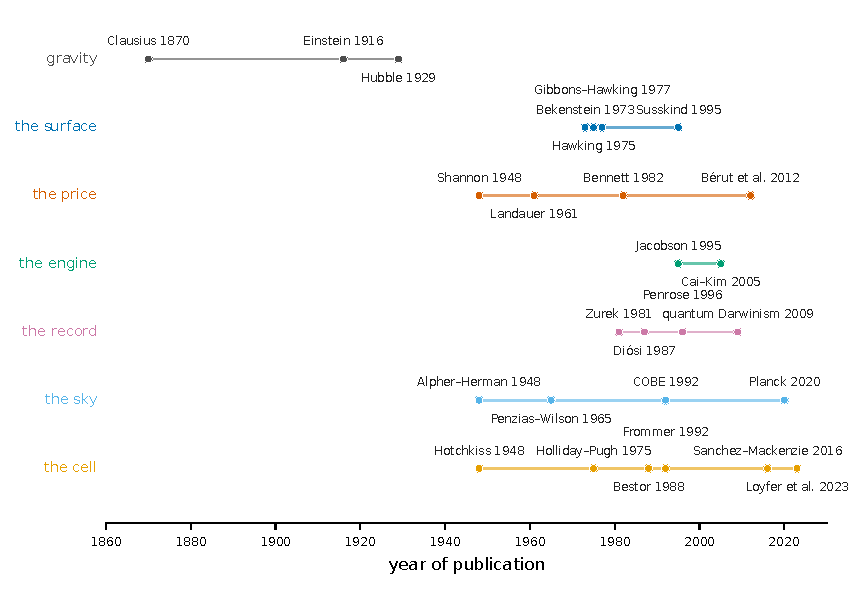
\includegraphics[width=\textwidth]{figures/front/fig_giants_timeline.pdf}
\caption{The threads IAM's Law is made of, by year of publication: gravity, the surface, the price of a bit, the engine, the record,
the sky and the cell. Each year is read from the book's bibliography by \texttt{figscripts/\allowbreak{}fig\_p0\_giants\_timeline.py}; the
span is 153 years, from Clausius's virial theorem (1870) to the atlas of purified human cell types (2023). \observed}\label{fig:giants}
\end{figure}}

\section*{Gravity: the half, the geometry and the expansion}

Clausius found the half~\cite{Clausius1870}. In a system bound by gravity and in equilibrium, the kinetic energy settles at half the
magnitude of the potential energy. \derived{} That theorem is older than every other piece here, and it sets the strength of the
informational term at the cosmic horizon: the coupling $\beta_m=\Omega_m/2$ is Clausius's half of the bound matter (Chapter~\ref{ch:virial}).

Einstein showed that gravity is not a force acting across empty space but the curvature of spacetime itself~\cite{Einstein1916}. Within
weeks of the field equations' appearance in November 1915, Karl Schwarzschild, serving in the artillery on the Russian front, found their
first exact solution~\cite{SchwarzschildGO}. At a critical radius the mathematics closed around the mass: an object crossing that boundary could never
return. Schwarzschild died in May 1916, at 42, months after sending the solution to Einstein, and never saw what it held. Decades later the
boundary he found was named a black hole.

In 1929 Hubble found that the galaxies recede at speeds proportional to their distance~\cite{Hubble1929}. \observed{} The universe was not
static. The rate he measured, the Hubble constant $H_0$, became one of the most contested numbers in science. In Part~\ref{part:2} it comes
out in two sectors of one posterior: $67.16$\,km\,s$^{-1}$\,Mpc$^{-1}$ for the photon sector, $72.26$ for the matter sector
(Chapter~\ref{ch:level2}). \measured{} (photon sector) \calc{} (matter sector)

\section*{The surface: entropy on the horizon}

By the early 1970s black holes had gone from a mathematical embarrassment to a reluctant acceptance, and they seemed to consume everything
and reveal nothing. Jacob Bekenstein, a graduate student under Wheeler at Princeton, asked a simple question: what happens to the second law
when something falls in? The object disappears behind the horizon with its entropy, and from outside the universe seems to have lost
entropy. His answer was that the black hole itself must carry entropy, proportional not to its volume or its mass but to the area of its
horizon~\cite{Bekenstein1973}. \derived{} Entropy had always been a property of matter. Bekenstein put it on a surface. The universe keeps
its books, and it keeps them on surfaces.

Stephen Hawking set out to show that a black hole could not have a temperature, since temperature implies radiation and nothing was supposed
to escape. Applying quantum field theory in curved spacetime, he found instead that black holes glow~\cite{Hawking1974,Hawking1975}. A black
hole radiates at a temperature set by its mass alone, $T_H=\hbar c^3/8\pi GMk_B$, about $6.2\times10^{-8}$\,K for one solar mass
(Chapter~\ref{ch:surfaces}). \derived{} The result joined gravity, quantum mechanics and thermodynamics in one equation, and it opened the
information problem that physics still debates. Gibbons and Hawking then gave the cosmological horizon the same thermodynamics: an
expanding universe has a horizon with an area, an entropy and a temperature, $T_{GH}=\hbar H/2\pi k_B$, about $2.65\times10^{-30}$\,K
today~\cite{GibbonsHawking1977}. \derived{} Unruh showed that an accelerated observer sees the vacuum as a thermal bath~\cite{Unruh1976},
and 't~Hooft and Susskind turned the area law into a principle: the information a region can hold is bounded by the area of its boundary,
not by its volume~\cite{tHooft1993,Susskind1995}.

These are the places of IAM. A horizon is a surface with a capacity, one unit of $k_B$ per four Planck areas, and a temperature. In the
language of this book it is an encoding surface (Chapter~\ref{ch:surfaces}).

\section*{The price: information is physical}

Claude Shannon never thought about black holes. He was an engineer at Bell Laboratories asking how to send a message through a noisy channel.
In 1948 he defined information mathematically, gave it a unit, the bit, and found the limits of any channel~\cite{Shannon1948}. His measure,
$H=-\sum_ip_i\log_2p_i$, has the form of the entropy of statistical mechanics. Every methylation reading in Part~\ref{part:4} is Shannon's
binary entropy $H(\beta)$ of a methylation level.

Rolf Landauer, at IBM in 1961, showed that erasing information costs energy~\cite{Landauer1961}. Not metaphorically: physically. Each time a
system goes from remembering a bit to not remembering it, at least $k_BT\ln2$ is dissipated as heat into an environment at temperature $T$.
\derived{} Thirty years later he put it in three words: information is physical~\cite{Landauer1991}. Charles Bennett completed the
argument~\cite{Bennett1982}. Computation can in principle be done reversibly and for free; the irreducible cost is the erasure. That is why
Maxwell's demon cannot win: to keep working it must clear its memory, and clearing it pays the price. The bound has since been measured, on a
colloidal particle in a double well~\cite{Berut2012} and on nanomagnetic bits~\cite{Hong2016}. \observed{} At body temperature it is
$2.97\times10^{-21}$\,J per bit (Chapter~\ref{ch:landauer}). \calc

Shannon gave information its mathematics. Landauer gave it a price. Bekenstein put it on horizons, and Hawking showed that those horizons
radiate. Every piece was on the table. What was missing was someone to notice that they fit together.

\section*{The engine: gravity from thermodynamics}

Bekenstein had put entropy on horizons and Hawking had shown that horizons radiate; the mathematics kept whispering that gravity and thermodynamics were the same thing, and no one had shown why. In 1995 Ted Jacobson asked what
happens if the argument is run backwards. Everyone had derived the thermodynamics of horizons from Einstein's equations. He started from
thermodynamics. He applied the Clausius relation $\delta Q=T\,dS$ to every local causal horizon, took the entropy proportional to the
horizon's area as Bekenstein had, and took the temperature to be Unruh's. Out came Einstein's field equations, in four
pages~\cite{Jacobson1995}. \derived{} Gravity is an equation of state: the macroscopic description of something happening at a deeper level,
as pressure and temperature describe molecules in a gas. Change the entropy functional and the field equations change with it. The
gravitational dynamics live in the entropy. Cai and Kim then showed that the same first law, applied at the apparent horizon of an expanding
universe, gives the Friedmann equations~\cite{CaiKim2005}. \derived

Jacobson's discovery was so powerful that the next question went unasked: what is the entropy made of? He used the geometric entropy alone,
and it gave general relativity. IAM adds one term to it: the classical records that matter writes as it decoheres, $S=S_{\rm geo}+S_{\rm
info}$ (Chapter~\ref{ch:theory}). \conjecture{} The Einstein equations are untouched; what changes is the entropy functional, the place
Jacobson showed the field equations live. Jacobson found the engine and showed that it runs on entropy. IAM names one of the fuels it was
burning all along.

Duration is the key. Matter travels on timelike worldlines: it has proper time, and decoherence takes time. Light travels on null geodesics,
$ds^2=0$, $\Delta\tau=0$: a photon experiences no proper time, does not decohere and writes no record. Given the identification, the split
between the two follows from the causal structure that general relativity already describes, not from an assumption. \derived{} Matter
feels a weaker effective coupling, $\mu<1$; light feels standard gravity, $\Sigma=1$; and the strength is Clausius's half,
$\beta_m=\Omega_m/2$, with nothing adjusted to the growth data. Nine Planck chains carry the coupling at its fixed value and are consistent with Planck; five
$\Lambda$CDM controls and four free-$\mu_0$ test chains run beside them (eighteen in all; Chapter~\ref{ch:dual}). \measured

\section*{The record: how the classical world is written}

Wojciech Zurek showed how a quantum system becomes a definite classical fact. The environment selects the states that survive, the pointer
states~\cite{Zurek1981}; superpositions of them decohere~\cite{JoosZeh1985,Zurek2003}; and the states that survive are those that leave many
redundant copies of themselves in the environment, so that observers who read any fragment agree on what they saw~\cite{Zurek2009}. \derived{}
The classical world is the set of records that decoherence leaves behind. Zurek showed how records form. IAM's Law prices each one.

John Wheeler, who named the black hole and supervised Bekenstein's thesis, distilled a lifetime of thinking about gravity and quantum
mechanics into three words: it from bit. Every physical quantity, he proposed, derives its meaning from answers to yes-or-no
questions~\cite{WheelerItFromBit}. \conjecture{} He could not formalize it, and he said it anyway. IAM's Law gives the phrase a price: no
bit becomes classical for free. \interp

Lajos Di\'osi and Roger Penrose asked whether gravity itself limits how long a mass can stay in two places at once. Di\'osi wrote a master
equation for gravitational decoherence~\cite{Diosi1987,Diosi1989}; Penrose argued that a superposition of two mass distributions reduces in a
time $\tau_{\rm DP}=\hbar/E_G$, where $E_G$ is the gravitational self-energy of their difference~\cite{Penrose1996}. \conjecture{} They put
gravity at the boundary between quantum and classical. IAM's Law, applied at the same boundary, gives a time set by the temperature of the
surface where the record is written. For a silica sphere of $10^{-12}$\,kg at 10\,mK the two pictures give $\tau_{\rm DP}=7.5\,\mu$s and
$\tau_{\rm IAM}=509$\,s, and doubling the temperature multiplies $\tau_{\rm IAM}$ by four while leaving $\tau_{\rm DP}$ unchanged
(Chapter~\ref{ch:quantumrecords}). \calc{} An underground search for the radiation the simplest version of their model implies has already
constrained it~\cite{Donadi2021}. \observed{} A superposition held at two bath temperatures separates the two pictures. \prediction

\section*{The sky: the instruments we borrowed}

In 1948 Alpher and Herman predicted that the hot early universe should have left a background of radiation, a few kelvin
today~\cite{AlpherHerman1948}. In 1961 E.~A.~Ohm, describing the Bell Laboratories receiver built for the Echo satellite, recorded a system
temperature 3.3\,K higher than its components accounted for~\cite{Ohm1961,Wilson1979}; the excess was small enough not to matter for the
project, and no one followed it up. In 1965 Penzias and Wilson, on the same horn antenna, measured an excess antenna temperature of about
3.5\,K that they could not remove~\cite{PenziasWilson1965}, and Dicke and his colleagues at Princeton, who were building an experiment to
look for it, recognized it as the radiation of the early universe~\cite{Dicke1965}. \observed{} The signal had been present and detectable
the whole time. What was missing was a precise enough instrument and knowing what to look for.

Then the analysts built the instruments. COBE measured the spectrum as a blackbody~\cite{Mather1994} and found the first variations across the
sky, about one part in $10^5$~\cite{Smoot1992}. The temperature is now known as 2.7255\,K~\cite{Fixsen2009}, and Planck mapped the variations over
the whole sky~\cite{Planck2018I,Planck2018VI}. \observed{} Along the way the field built the tools this book uses: HEALPix to put data on a
sphere in pixels of equal area~\cite{Gorski2005}; CAMB to compute the spectra~\cite{Lewis2000CAMB}; the $\mu$--$\Sigma$ language for
gravity that treats matter and light separately~\cite{PogosianSilvestri2016} and MGCAMB to compute it~\cite{Zhao2009MGCAMB,Wang2023MGCAMB};
Cobaya to sample the likelihood~\cite{Torrado2021}; and convergence diagnostics that say when a chain can be trusted~\cite{Gelman1992}.

The tools have changed who can use them. The Planck 2018 likelihood is public; CAMB, MGCAMB and Cobaya are open. Because the analysts gave
their tools away, the chains of Part~\ref{part:2} could be run by an independent researcher, without institutional permission. The barriers
to serious cosmology used to be the tools themselves. Those barriers are gone, and the people who removed them are among the giants of this
chapter. Part~\ref{part:4} carries the same tools to the cell (Chapter~\ref{ch:skytools}).

\section*{The cell: a record copied at every division}

In 1944 Erwin Schr\"odinger asked how a living cell keeps its order against the thermal noise that should scramble it~\cite{SchrodingerWhatIsLife}.
He proposed that heredity is carried by an ``aperiodic crystal'' and that an organism stays alive by drawing order from its surroundings.
\conjecture{} The question in the subtitle of this book, the energy that holds the classical world against thermal noise, is his question asked
of a record. \interp

The record was found by biochemists. Rollin Hotchkiss separated a fifth base from calf thymus DNA by paper chromatography in 1948, the
methylated cytosine~\cite{Hotchkiss1948}. \observed{} In 1975 Holliday and Pugh, and independently Riggs, proposed that a pattern of
methylation could be inherited: an enzyme that recognizes a CpG methylated on one strand only would restore the mark on the new strand after
each division, so that a cell's identity is written in a pattern and copied~\cite{HollidayPugh1975,Riggs1975}. The copying enzyme was cloned
by Bestor and colleagues~\cite{Bestor1988}; the enzymes that write new marks were found by Okano and colleagues~\cite{Okano1999}; and UHRF1
was shown to bring the copying enzyme, DNMT1, to the hemimethylated sites at the replication fork~\cite{Bostick2007,Sharif2007}. \observed{}
Hopfield had already shown that any copy made with a finite free-energy discrimination makes errors in proportion to a Boltzmann factor, and
that proofreading can lower them at a cost~\cite{Hopfield1974}. \derived{} Genereux and colleagues measured the fidelity of the copy, site by
site, from both strands of single molecules~\cite{Genereux2005}. \observed

Others made the record readable. Bisulfite sequencing turned each methylated cytosine into a letter that can be read~\cite{Frommer1992};
human methylomes were read at single-base resolution~\cite{Lister2009}; the arrays that Part~\ref{part:4} reads were built and characterized
by their makers~\cite{Bibikova2011,Pidsley2016}; reference methods separated the cells in a blood specimen~\cite{Houseman2012,Salas2018}; and
an atlas of purified healthy human cell types gave read-level data on which a copy error can be counted molecule by
molecule~\cite{Loyfer2023}. \observed{} Feinberg and Vogelstein found in 1983 that the methylation of cancer cells departs from that of the
normal cells they came from~\cite{FeinbergVogelstein1983}, and four decades of work since have mapped how the cancer epigenome
differs~\cite{Baylin2011}. \observed

What IAM adds here is the floor. A cell holds each maintained site against thermal noise with a holding energy of $3.41\,\kB T$, measured on
single molecules of healthy cells (\measured); the form of the floor, $\varepsilon_0=1/(1+e^{E_{\rm hold}/\kB T})=0.032$, follows from a
Boltzmann factor (\derived); and the cell's copy error is read against it (Chapter~\ref{ch:iama}).

\section*{Sanchez and Mackenzie: the bridge crossed before}

The first to put Landauer's bound on methylation were Sanchez and Mackenzie~\cite{Sanchez2016}. They treated a change in methylation at a
region of the genome as information processing, priced it at $\kB T\ln2$ per bit, showed that the thermal background of methylation change
follows a Weibull distribution whose scale recovers the persistence length of DNA from methylome data alone, and in 2019 turned this into a
method for separating regulatory signal from that background~\cite{Sanchez2019}. \observed{} We came to the same bridge from the
thermodynamics of bound systems and read their work only after our reference values were first frozen. Their crossing from Landauer to the
methylome came first, and this chapter records it. They use $\kB T$ as the scale of a
background to be filtered; Part~\ref{part:4} uses it as the unit of measure. One filters; the other calibrates. The two are complementary
(Chapter~\ref{ch:landauer}).

\section*{The thread is still giving}

Clausius found the half. Einstein showed that falling is geometry, and Schwarzschild found a horizon hiding in the geometry. Hubble found the
expansion. Bekenstein put entropy on the horizon, and Hawking, Gibbons and Unruh gave the horizon a temperature. Shannon gave information its
mathematics, and Landauer and Bennett gave it a price. Jacobson, and Cai and Kim, showed that the entropy writes the field equations. Zurek
showed how records form, and Di\'osi and Penrose asked what gravity has to do with it. The analysts of the sky built the instruments and gave
them away. The biochemists found the record in the cell and the enzymes that copy it, and Sanchez and Mackenzie first priced it.

Each one handed something to the next without knowing it. Each one was missing the piece that the others had. The missing piece was not a
new particle, a new dimension or a new force. It was not hiding in a collider or a supercomputer center. The missing information was always
information.

If IAM is right, it is one more brick, placed where the architecture always left room for it. The predictions are dated
(Chapter~\ref{ch:predictions}). The growth surveys are the next test of the matter coupling, and the decisive one is the turn-on of the growth ramp
(Section~\ref{sec:sp_euclid}). \prediction{} The prediction is on the table, waiting
for the data. The thread is still giving.
